\documentclass[11pt,a4paper]{article}
\newcommand{\gls}[1]{#1\textsubscript{G}}
\usepackage[utf8]{inputenc}
\usepackage[italian]{babel}
\usepackage{geometry}
\usepackage{graphicx}
\usepackage{float}
\usepackage{tabularx}
\usepackage{booktabs}
\usepackage{caption}
\usepackage{hyperref}
\usepackage{fancyhdr}
\usepackage{lastpage}
\usepackage{longtable}

\usepackage{array}
\newcolumntype{M}[1]{>{\centering\arraybackslash}m{#1}}

\geometry{margin=2.5cm}

% Intestazione e piè di pagina
\pagestyle{fancy}
\fancyhf{}
\renewcommand{\headrulewidth}{0pt}
\fancyfoot[C]{\thepage\ di \pageref{LastPage}}

\begin{document}

% Prima pagina - Intestazione
\begin{titlepage}
    \centering
    
    % Logo Università
    \begin{figure}[H]
        \centering
        
\includegraphics[width=0.3\textwidth]{../logoUnipd.jpg}
    \end{figure}
    
    \vspace{0.5cm}
    
    \textbf{\Large Università degli Studi di Padova} \\
    \vspace{0.2cm}
    \textbf{Laurea in Informatica} \\
    \vspace{0.2cm}
    \textbf{Corso di Ingegneria del Software} \\
    \vspace{0.2cm}
    \textbf{Anno Accademico 2025/2026} \\
    
    \vspace{1cm}
    
    % Logo gruppo
    \begin{figure}[H]
        \centering
        
\includegraphics[width=0.2\textwidth]{../LogoByteMe.jpg}
    \end{figure}
    
    \vspace{0.5cm}
    
    \textbf{\Large Gruppo ByteMe} \\
    \vspace{0.2cm}
    \texttt{byteme2025swe@gmail.com} \\
    
    \vspace{1cm}
    
    \textbf{\Huge \gls{Specifica Tecnica}} \\
    
    \vspace{1.5cm}
    
    \begin{table}[H]
        \centering
        \begin{tabular}{|l|p{5cm}|}
            \hline
            \textbf{Versione} & 0.1.1 \\
            \hline
            \textbf{Stato} & In corso \\
            \hline
            \textbf{Redazione} & Giulia Barzon, Joseph Grant, Chiara Grossele, Matteo Cuogo \\
            \hline
            \textbf{\gls{Verifica}} & Da verificare\\
            \hline
            \textbf{Approvazione} & Da approvare\\
            \hline
            \textbf{Proprietario} & ByteMe \\
            \hline
            \textbf{Uso} & Esterno \\
            \hline
            \textbf{Destinatari} & Prof. Tullio Vardanega \\ & Prof. Riccardo Cardin \\
            \hline
        \end{tabular}
    \end{table}
    
    \vfill
\end{titlepage}

% Seconda pagina - Versionamento
\thispagestyle{empty}
\section*{Registro dei Cambiamenti}

\begin{table}[H]
    \centering          
    \begin{tabular}{|c|c|c|>{\raggedright\arraybackslash}p{0.35\textwidth}|p{0.18\textwidth}|}
        \hline
        \textbf{Versione} & \textbf{Data} & \textbf{Autore} & \textbf{Descrizione} & \textbf{\gls{Verifica}} \\
        \hline
        0.1.2 & 22/04/2026 & Elisa marchioro & Sistemata sezione architettura del backend & \\
        \hline
        0.1.1 & 21/04/2026 & Giulia Barzon & Struttura documento e sezione MVVM, bozza del Facade & Chiara Grossele, Elisa Marchioro\\
        \hline
        0.1.0 & 21/04/2026 & Giulia Barzon & Completate sezione 1, 2 e 3 & Chiara Grossele, Elisa Marchioro\\
        \hline
        0.0.10 & 20/04/2026 & Elisa Marchioro & Fix alle tabelle & Giulia Barzon\\
        \hline
        0.0.9 & 20/04/2026 & Giulia Barzon & Mappatura requisiti soddisfatti (una parte) & Elisa Marchioro\\
        \hline
        0.0.8 & 18/04/2026 & Joseph Grant & Aggiunti i hook frontend & Elisa Marchioro\\
        \hline
        0.0.7 & 18/04/2026 & Matteo Cuogo & Aggiunta pattern Registry & Giulia Barzon, Elisa Marchioro\\
        \hline
        0.0.6 & 17/04/2026 & Matteo Cuogo & Aggiunta sezione Design Pattern & Giulia Barzon, Elisa Marchioro\\
        \hline
        0.0.5 & 17/04/2026 & Chiara Grossele & Aggiunta sezione Tracciamento dei requisiti & Matteo Cuogo, Elisa Marchioro\\
        \hline
        0.0.4 & 17/04/2026 & Joseph Grant & Aggiunta descrizione delle componenti frontend & Chiara Grossele, Matteo Cuogo\\
        \hline
        0.0.3 & 15/04/2026 & Chiara Grossele & Modifica struttura e aggiunte alla sezione Architettura backend & Joseph Grant, Matteo Cuogo, Giulia Barzon \\
        \hline
        0.0.2 & 14/04/2026 & Joseph Grant & Aggiunta tecnologie e architettura & Chiara Grossele, Giulia Barzon\\
        \hline
        0.0.1 & 28/03/2026 & Giulia Barzon & Creazione del documento, scrittura introduzione & Tommaso Tombacco \\
        \hline
    \end{tabular}
    \caption{Registro delle versioni del documento}
    \label{tab:versionamento}
\end{table}
\newpage

% Terza pagina - Indice
\tableofcontents
\thispagestyle{empty}
\newpage

% Dalla quarta pagina - Contenuto principale
\setcounter{page}{1}

\section{Introduzione}
\subsection{Scopo del documento}
Il presente documento costituisce la \textbf{\gls{Specifica Tecnica}} del prodotto
\textit{Second Brain}, proposto dall'azienda \textit{Zucchetti} al
gruppo ByteMe.
 
Il documento descrive in dettaglio:
\begin{itemize}
  \item le \textbf{tecnologie} adottate (linguaggi, framework, librerie, strumenti);
  \item l'\textbf{architettura} logica e fisica del sistema, con i pattern architetturali scelti;
  \item i \textbf{design pattern} applicati a livello di componenti, con motivazione delle scelte;
  \item la \textbf{documentazione \gls{API}} tra frontend e backend;
  \item i \textbf{requisiti soddisfatti} con riferimento al documento \textit{\gls{Analisi dei Requisiti}} v2.0.0.
\end{itemize}
 
Il documento è rivolto al team di sviluppo come guida implementativa e a
committente e proponente come \gls{verifica} della coerenza tra scelte progettuali e requisiti concordati.
 
\subsection{Approccio alla redazione}
Il documento viene redatto in modo \textbf{incrementale}, assicurando coerenza con gli sviluppi in corso. Non puo essere considerato completo fino al rilascio della versione 1.0.0.

\subsection{Scopo del prodotto}
Il progetto \textit{Second Brain} mira a sviluppare un \gls{editor di testo} avanzato basato sul linguaggio \gls{Markdown} e potenziato dall'integrazione di Large Language Model (LLM).
L'applicazione web consentira all'utente di:
\begin{itemize}
  \item scrivere e visualizzare in tempo reale testi formattati in \gls{Markdown};
  \item interagire con un LLM per riassumere, correggere, riscrivere e tradurre testi;
  \item ottenere analisi critiche multi-prospettiche secondo il metodo dei \textit{Sei Cappelli per Pensare} di Edward De Bono;
  \item delegare all'AI la stesura completa di un testo tramite \gls{Distant Writing}.
\end{itemize}
 
\subsection{\gls{Glossario}}
Per evitare ambiguità, i termini tecnici usati nel documento vengono definiti in modo più approfondito nel documento \gls{Glossario} v2.0.0 che si può trovare nel sito web del gruppo ByteMe alla sezione Documenti Interni e raggiungibile dal seguente link:\\
\href{https://byteme25.github.io/ByteMe/files.html}{ByteMe/\gls{Glossario} v2.0.0}

I termini che vengono considerati meritevoli di approfondimenti sono indicati con una G a pedice.


\subsection{Riferimenti}
\begin{itemize}
  \item \textit{\gls{Norme di Progetto}} versione 2.0.0\\
  \href{https://byteme25.github.io/ByteMe/files.html}{ByteMe/\gls{Norme di Progetto} v2.0.0}
  \item Capitolato d'appalto C6: \textit{Second Brain} (Zucchetti S.p.A.)\\ \url{https://www.math.unipd.it/~tullio/IS-1/2025/Progetto/C6.pdf}
  \item Regolamento del progetto didattico:\\
        \url{https://www.math.unipd.it/~tullio/IS-1/2023/Dispense/PD2.pdf}
\end{itemize}
 
\subsubsection{Riferimenti informativi}
\begin{itemize}
    \item \textit{\gls{Analisi dei Requisiti}} versione 2.0.0 (Ultimo accesso: 20/04/2026)\\
    \href{https://byteme25.github.io/ByteMe/}{PB - \gls{Analisi dei Requisiti} v2.0.0}
    \item \textit{Piano di Qualifica} versione 2.0.0 (Ultimo accesso: 20/04/2026) \\
    \href{https://byteme25.github.io/ByteMe/}{PB - Piano di Qualifica v2.0.0}
    \item Verbali interni ed esterni
    \item \gls{Glossario} versione 2.0.0 (Ultimo accesso: 20/04/2026)\\
    \href{https://byteme25.github.io/ByteMe/files.html}{Documenti interni - \gls{Glossario} v2.0.0}
    \item \gls{Repository} ufficiale di \gls{EasyMDE}: \url{https://github.com/Ionaru/easy-markdown-editor}\\ (Ultimo accesso: 24/03/2026)
     \item Documentazione linguaggio \gls{markdown} - CommonMark: \url{https://commonmark.org/}\\ (Ultimo accesso: 20/02/2026)
    \item Documentazione \gls{React} 19: \url{https://react.dev}\\ (Ultimo accesso: 16/04/2026)
    \item Principi del Bulletproof \gls{React} (\gls{repository} ufficiale): \url{https://github.com/alan2207/bulletproof-react}\\ (Ultimo accesso: 16/04/2026)
    \item Documentazione \gls{Flask}: \url{https://flask.palletsprojects.com}\\ (Ultimo accesso: 10/03/2026)
    \item Documentazione \gls{Docker}: \url{https://docs.docker.com}\\ (Ultimo accesso: 27/02/2026)
    \item Documentazione TypeScript: \url{https://www.typescriptlang.org/docs/}\\ (Ultimo accesso: 27/03/2026)

    \item Slide del corso di Ingegneria del Software\\ (Ultimo accesso: 10/04/2026)
    \item Principi SOLID (slide prof. Cardin)
    \item Pattern architetturali (slide prof. Cardin)
\end{itemize}

\newpage

\section{Tecnologie}
\subsection{Framework frontend}
\begin{table}[H]
    \centering
    \begin{tabular}{|p{0.20\textwidth}|p{0.10\textwidth}|p{0.55\textwidth}|}
        \hline
        \textbf{Nome} & \textbf{Versione} & \textbf{Descrizione} \\
        \hline
        \gls{React} & 19.2.0 & Libreria JavaScript per la costruzione di interfacce utente basate su componenti riutilizzabili. \\
        \hline
    \end{tabular}
    \caption{Descrizione del framework frontend}
    \label{tab:framework_frontend}
\end{table}

\subsection{Librerie frontend}
\begin{table}[H]
    \centering
    \begin{tabular}{|p{0.20\textwidth}|p{0.10\textwidth}|p{0.55\textwidth}|}
        \hline
        \textbf{Nome} & \textbf{Versione} & \textbf{Descrizione} \\
        \hline
        \gls{EasyMDE} & 2.20.0 & Editor \gls{Markdown} con anteprima in tempo reale, basato su CodeMirror. \\
        \hline
        Axios & 1.7.9 & Client HTTP basato su Promise per effettuare richieste REST dal browser. \\
        \hline
        \gls{React Router} DOM & 7.13.1 & Libreria standard per il routing dichiarativo in applicazioni \gls{React}, utilizzata per la navigazione tra le viste. \\
        \hline
        \gls{Zustand} & 5.0.12 & Libreria di state management leggera, utilizzata per la gestione dello stato globale e la persistenza dei dati nel LocalStorage. \\
        \hline
        Lucide-\gls{React} & 1.8.0 & Libreria di icone vettoriali utilizzata per la UI dell'applicazione. \\
        \hline
        \gls{React} Hot Toast & 2.6.0 & Libreria leggera per la visualizzazione di notifiche toast personalizzabili. \\
        \hline
        \gls{CSS Modules} & N/A (Integrato) & Sistema di scope locale per i fogli di stile CSS integrato in \gls{Vite}, che evita conflitti tra classi. \\
        \hline
        ESLint & 9.39.1 & Strumento di linting per TypeScript, che aiuta a mantenere uno stile di codice coerente e a individuare errori. \\
        \hline
    \end{tabular}
    \caption{Descrizione delle librerie frontend}
    \label{tab:librerie_frontend}
\end{table}

\subsection{Linguaggio frontend}
\begin{table}[H]
    \centering
    \begin{tabular}{|p{0.20\textwidth}|p{0.10\textwidth}|p{0.55\textwidth}|}
        \hline
        \textbf{Nome} & \textbf{Versione} & \textbf{Descrizione} \\
        \hline
        TypeScript & 5.9.3 & Superset tipizzato di JavaScript che aggiunge tipizzazione statica e migliora la manutenibilità del codice. \\
        \hline
        TSX & N/A (Sintassi) & Estensione di TypeScript che consente di scrivere markup \gls{JSX} all'interno di file tipizzati, usata per i componenti \gls{React}. \\
        \hline
    \end{tabular}
    \caption{Descrizione dei linguaggi frontend}
    \label{tab:linguaggi_frontend}
\end{table}

\subsection{Tecnologie di build e runtime}
\begin{table}[H]
    \centering
    \begin{tabular}{|p{0.20\textwidth}|p{0.10\textwidth}|p{0.55\textwidth}|}
        \hline
        \textbf{Nome} & \textbf{Versione} & \textbf{Descrizione} \\
        \hline
        \gls{Vite} & 7.3.1 & Build tool moderno e veloce per applicazioni web, con supporto nativo a ES modules e Hot Module Replacement. \\
        \hline
        Node.js & 20-alpine & Ambiente di runtime JavaScript lato server, utilizzato nel \gls{Dockerfile} per la fase di compilazione del frontend. \\
        \hline
    \end{tabular}
    \caption{Descrizione delle tecnologie di build}
    \label{tab:tecnologie_build}
\end{table}

\subsection{Tecnologie di test}
\begin{table}[H]
    \centering
    \begin{tabular}{|p{0.20\textwidth}|p{0.10\textwidth}|p{0.55\textwidth}|}
        \hline
        \textbf{Nome} & \textbf{Versione} & \textbf{Descrizione} \\
        \hline
        \gls{Vitest} & 4.1.4 & Framework di testing per applicazioni \gls{Vite}, compatibile con l'\gls{API} di Jest e ottimizzato per TypeScript. \\
        \hline
        \gls{Pytest} & 7.0.0 & Framework di testing per Python, con sintassi semplice e supporto a fixture, parametrizzazione e plugin. \\
        \hline
        \gls{React} testing library & 16.3.2 & Libreria per il testing di componenti \gls{React}, che fornisce utilities per interagire con i componenti in modo simile a come un utente reale lo farebbe. \\
        \hline
    \end{tabular}
    \caption{Descrizione delle tecnologie di test}
    \label{tab:tecnologie_test}
\end{table}

\subsection{Framework \gls{API} backend}
\begin{table}[H]
    \centering
    \begin{tabular}{|p{0.20\textwidth}|p{0.10\textwidth}|p{0.55\textwidth}|}
        \hline
        \textbf{Nome} & \textbf{Versione} & \textbf{Descrizione} \\
        \hline
        \gls{Flask} & 3.1.3 & Microframework Python per lo sviluppo di \gls{API} REST, leggero ed estensibile tramite plugin. \\
        \hline
    \end{tabular}
    \caption{Descrizione del framework \gls{API} backend}
    \label{tab:api_backend}
\end{table}

\subsection{Linguaggio backend}
\begin{table}[H]
    \centering
    \begin{tabular}{|p{0.20\textwidth}|p{0.10\textwidth}|p{0.55\textwidth}|}
        \hline
        \textbf{Nome} & \textbf{Versione} & \textbf{Descrizione} \\
        \hline
        Python & 3.12-slim & Linguaggio di programmazione ad alto livello, utilizzato per la logica di business e l'implementazione delle \gls{API}. \\
        \hline
    \end{tabular}
    \caption{Descrizione del linguaggio backend}
    \label{tab:linguaggio_backend}
\end{table}

\subsection{Librerie backend}
\begin{table}[H]
    \centering
    \begin{tabular}{|p{0.20\textwidth}|p{0.10\textwidth}|p{0.55\textwidth}|}
        \hline
        \textbf{Nome} & \textbf{Versione} & \textbf{Descrizione} \\
        \hline
        OpenAI & 2.31.0 & Libreria ufficiale utilizzata per l'integrazione e la comunicazione con le \gls{API} dei modelli linguistici (LLM). \\
        \hline
        Pydantic & 2.12.5 & Libreria per la \gls{validazione} dei dati e la serializzazione tramite annotazioni di tipo nativo in Python. \\
        \hline
        \gls{Flask}-CORS & 6.0.2 & Estensione di \gls{Flask} per la gestione sicura del Cross-Origin Resource Sharing tra frontend e backend. \\
        \hline
        Python-dotenv & 1.2.2 & Modulo per il caricamento delle variabili d'ambiente e chiavi \gls{API} dai file \texttt{.env}. \\
        \hline
    \end{tabular}
    \caption{Descrizione delle librerie backend}
    \label{tab:librerie_backend}
\end{table}

\subsection{Server Web}
\begin{table}[H]
    \centering
    \begin{tabular}{|p{0.20\textwidth}|p{0.10\textwidth}|p{0.55\textwidth}|}
        \hline
        \textbf{Nome} & \textbf{Versione} & \textbf{Descrizione} \\
        \hline
        \gls{Nginx} & alpine & Server web ad alte prestazioni utilizzato nel container \gls{Docker} per servire i file statici del frontend e gestire il routing. \\
        \hline
        Werkzeug & 3.1.8 & Server WSGI integrato in \gls{Flask}, utilizzato attualmente come motore di esecuzione per l'ambiente backend. \\
        \hline
    \end{tabular}
    \caption{Descrizione dei server web frontend e backend}
    \label{tab:server_web}
\end{table}

\subsection{Tecnologie deployment}
\begin{table}[H]
    \centering
    \begin{tabular}{|p{0.20\textwidth}|p{0.10\textwidth}|p{0.55\textwidth}|}
        \hline
        \textbf{Nome} & \textbf{Versione} & \textbf{Descrizione} \\
        \hline
        \gls{Docker} & 29.4.0 & Piattaforma per la containerizzazione, utilizzata per isolare frontend e backend in ambienti riproducibili. \\
        \hline
        \gls{Docker Compose} & 5.1.2 & Strumento per definire e gestire applicazioni multi-container tramite il file \texttt{\gls{docker}-compose.yml}. \\
        \hline
    \end{tabular}
    \caption{Descrizione delle tecnologie di deployment}
    \label{tab:tecnologie_deployment}
\end{table}

\newpage

\section{Infrastruttura e deployment}
Il sistema \textit{Second Brain} utilizza la tecnologia di containerizzazione \textbf{\gls{Docker}} per garantire l'isolamento dei componenti, la portabilità tra diversi ambienti di sviluppo e produzione e la gestione semplificata delle dipendenze.

\subsection{Strategia di containerizzazione}
L'architettura è suddivisa in due micro-servizi orchestrati tramite \texttt{\gls{docker}-compose}, che permette di definire reti virtuali interne e volumi per la persistenza o il \textit{hot-reloading} durante lo sviluppo.

\subsection{Backend (\gls{Flask})}
Il container del backend è ottimizzato per l'esecuzione di script Python in un ambiente leggero e sicuro.
\begin{itemize}
    \item \textbf{Immagine di base}: \texttt{python:3.12-slim}. La scelta della variante \textit{slim} riduce l'ingombro dell'immagine, contenendo solo le librerie essenziali per il runtime Python 3.12.
    \item \textbf{Configurazione}: La directory di lavoro è impostata su \texttt{/app}. Il sistema installa le dipendenze tramite \texttt{pip} senza utilizzare la cache per mantenere l'immagine snella.
    \item \textbf{Networking}: Il container espone la porta \texttt{8000}.
    \item \textbf{Variabili d'ambiente}: Il backend riceve dinamicamente tramite il file \texttt{.env} le chiavi necessarie per il funzionamento degli LLM.
\end{itemize}

\subsection{Frontend (\gls{React} + \gls{Nginx})}
Per il frontend è stata adottata una strategia di \textbf{Multi-stage Build}, che separa l'ambiente di compilazione da quello di esecuzione.
\begin{itemize}
    \item \textbf{Stage 1 (Build)}: Utilizza \texttt{node:20-alpine} per installare le dipendenze ed eseguire la build di produzione tramite \gls{Vite}. L'uso di Alpine Linux garantisce velocità e leggerezza nel processo di CI/CD.
    \item \textbf{Stage 2 (Production)}: Il risultato della build viene copiato in un'immagine \texttt{\gls{nginx}:alpine}. \gls{Nginx} funge da web server statico ad alte prestazioni, configurato appositamente per gestire il routing \textit{client-side} tipico delle Single Page Application (SPA).
\end{itemize}

\subsection{Orchestrazione: \gls{Docker Compose}}
Il file \texttt{\gls{docker}-compose.yml} coordina l'avvio sincronizzato dei servizi e la gestione delle risorse:
\begin{itemize}
    \item \textbf{Mapping delle porte}: Il frontend è reso accessibile all'host sulla porta \texttt{8080}, mappata sulla porta interna \texttt{80} di \gls{Nginx}.
    \item \textbf{Dipendenze}: È definita una clausola \texttt{depends\_on} che assicura che il container del backend sia avviato prima di quello del frontend.
    \item \textbf{Sviluppo \gls{Agile}}: Durante la fase di sviluppo, viene utilizzato un \textit{bind mount} per permettere al server \gls{Flask} di riflettere istantaneamente le modifiche al codice senza dover ricostruire l'immagine.
\end{itemize}

% immagine rappresentativa dell'ambiente docker
\begin{figure}[H]
    \centering
    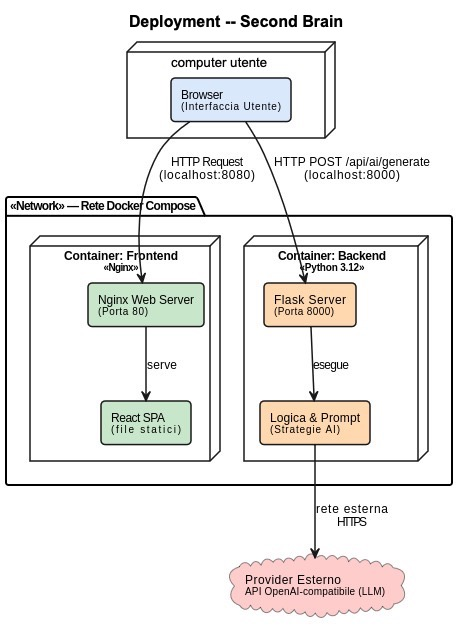
\includegraphics[width=0.9\textwidth]{../UMLimg/imgDocker.jpg}
    \caption{Rappresentazione dell'architettura di deployment tramite \gls{Docker Compose}}
    \label{fig:architettura_deployment}
\end{figure}


\newpage

\section{Architettura del backend}
Il sistema \textit{Second Brain} adotta il pattern architetturale \textbf{Layered Architecture} per il backend. L'adozione di questa struttura garantisce una netta separazione delle responsabilità e riduce l'accoppiamento tra i moduli software. Il flusso di esecuzione è strettamente unidirezionale (top-down): ogni strato funge da astrazione per quello superiore, gestendo esclusivamente la logica di propria competenza. Coerentemente con i requisiti di progetto, il backend è progettato per essere \textbf{stateless}, delegando la persistenza dei dati interamente al client. L'architettura logica si articola nei seguenti livelli:
\begin{itemize}
\item \textbf{Presentation Layer}: Espone gli endpoint REST, riceve le richieste HTTP e restituisce le risposte al client;
\item \textbf{Business Logic}: Core funzionale del sistema, contiene le regole di dominio e orchestra le operazioni tramite il pattern Strategy;
\item \textbf{Infrastructure Layer}: Gestisce la comunicazione con i provider LLM esterni e la post-elaborazione delle risposte.
\end{itemize}

\subsection{Presentation layer (app.py)}
Rappresenta il punto di ingresso del backend ed è implementato nel modulo di routing di Flask. Ha il compito di esporre gli endpoint REST, ricevere le richieste HTTP in ingresso e restituire risposte JSON standardizzate al client. Questo strato non contiene logica di dominio né conoscenza dei prompt o dei modelli LLM: si limita a validare i payload in ingresso e delegare l'elaborazione agli strati sottostanti.

\subsection{Business logic (ai\_strategies.py, operation\_registry.py)}
È il nucleo funzionale del sistema, completamente isolato dal framework web e dal protocollo HTTP. Utilizza il pattern comportamentale Strategy per gestire la variabilità delle operazioni in modo estensibile.

I componenti principali sono:
\begin{itemize}
\item \textbf{ai\_strategies.py} - gestione dei prompt: definisce come costruire i prompt per ogni operazione. Ogni strategia incapsula le istruzioni e la temperatura adatta al tipo di elaborazione richiesta, che sia un'operazione editoriale, una traduzione o un'analisi con i Sei Cappelli di De Bono.
\item \textbf{operation\_registry.py} - mappatura delle operazioni: contiene una mappatura statica che associa ogni identificatore di operazione alla strategia di prompt e al modello LLM corretto tramite oggetti OperationConfig. Funge da punto di configurazione centrale del sistema.
\end{itemize}

\subsection{Infrastructure layer}
Gestisce tutto ciò che riguarda il mondo esterno al dominio applicativo, isolando il resto del sistema dalle complessità di rete e di post-elaborazione.

I componenti principali sono:
\begin{itemize}
\item \textbf{model\_strategies.py} — integrazione modelli LLM: astrae la comunicazione con i provider esterni tramite l'interfaccia AIModelStrategy, esponendo i modelli Llama 3.2 e Gemma 3 in modo polimorfico. Gestisce l'iniezione delle variabili d'ambiente necessarie.
\item \textbf{text\_cleaning.py} — servizi di supporto: pulisce le risposte dei modelli rimuovendo metatesto e preamboli indesiderati tramite espressioni regolari.
\end{itemize}

\subsection{Descrizione delle classi}

\subsubsection{ai\_strategies.py}
Questo file contiene la logica di costruzione dei prompt tramite il pattern Strategy.

\paragraph{BaseAIStrategy} 
BaseAIStrategy è la classe astratta base del modulo. Dichiara la temperatura di default, fornisce il metodo \_validate() per la validazione dell'input e impone alle sottoclassi l'implementazione del metodo build(), che restituisce la coppia (system\_prompt, user\_prompt).
\begin{itemize}

\item \textbf{Attributi}:

\begin{itemize}
\item temperature: attributo che definisce il grado di creatività della risposta del modello AI. Il valore di default è 0.5, sovrascrivibile nelle sottoclassi in base all'operazione.
\end{itemize}

\item \textbf{Metodi}: 

\begin{itemize}
\item \_validate(): metodo concreto ereditabile che verifica che il testo in ingresso non sia None, sollevando un TypeError in caso contrario.
\item build(): metodo astratto che ogni sottoclasse deve implementare. Riceve il testo da elaborare e restituisce la coppia (system\_prompt, user\_prompt) da passare al modello LLM.
\end{itemize}


\end{itemize}

\paragraph{SimplePromptStrategy} 
SimplePromptStrategy è la strategia generica per operazioni editoriali standard. La temperatura è 0.5.
\begin{itemize}

\item \textbf{Attributi}:

\begin{itemize}
\item role: stringa che definisce il ruolo assegnato al modello nel system prompt.
\item task: stringa che definisce l'istruzione specifica inserita nello user prompt.
\end{itemize}

\item \textbf{Metodi}: 

\begin{itemize}
\item build(): combina role e task con il testo in ingresso, costruendo un system prompt e user prompt con l'istruzione specifica.
\end{itemize}


\end{itemize}

\paragraph{TranslationStrategy} 
TranslationStrategy è la strategia specializzata per le traduzioni. La temperatura è 0.3, ridotta per favorire fedeltà al testo originale.
\begin{itemize}

\item \textbf{Attributi}:

\begin{itemize}
\item language: stringa che definisce la lingua della traduzione.
\end{itemize}

\item \textbf{Metodi}: 

\begin{itemize}
\item build(): costruisce un system prompt ottimizzato per la traduzione professionale e un user prompt che specifica la lingua e il testo da tradurre.
\end{itemize}


\end{itemize}

\paragraph{DeBonoHatStrategy} 
DeBonoHatStrategy è la strategia specializzata per i Sei Cappelli di De Bono. Riceve tutti i parametri di configurazione nel costruttore, permettendo di definire un comportamento completamente personalizzato per ciascun cappello.
\begin{itemize}

\item \textbf{Attributi}:

\begin{itemize}
\item \_system\_prompt: system prompt preconfigurato che definisce la prospettiva del cappello.
\item \_user\_task: istruzione strutturata che guida il modello nella produzione di un output organizzato per punti.
\item temperature: sovrascrive il valore di default della classe base. Usiamo valori bassi (0.1) per i cappelli analitici (bianco, nero, blu) e valori alti (0.8) per i cappelli creativi ed emotivi (rosso, giallo, verde).
\end{itemize}

\item \textbf{Metodi}: 

\begin{itemize}
\item build(): combina \_user\_task con il testo in ingresso nel user prompt, restituendo la coppia con il system prompt preconfigurato.
\end{itemize}

\end{itemize}

\paragraph{STRATEGIES}
STRATEGIES è il dizionario statico che raccoglie tutte le istanze delle strategie di prompt disponibili nel sistema, indicizzate per identificatore di operazione (es. "summary", "black\_hat", "translate\_en"). Serve da sorgente da cui OPERATION\_REGISTRY attinge per comporre i propri OperationConfig.

\subsubsection{operation\_registry.py}
Questo file contiene la struttura dati OperationConfig, un dataclass che accoppia una strategia di prompt con una classe di modelli AI. Il dizionario OPERATION\_REGISTRY costituisce la mappatura statica centrale del sistema: associa ogni identificatore di operazione (es. "summary", "black\_hat", "translate\_en") al corrispondente OperationConfig. Funge da punto di configurazione centrale, rendendo l'aggiunta di nuove operazioni una modifica localizzata.

\paragraph{OperationConfig}
Dataclass che accoppia una strategia di prompt con una classe di modelli AI.
\begin{itemize}
\item model\_class: riferimento alla classe del modello LLM da istanziare per l'operazione.
\item prompt\_strategy: istanza della strategia di prompt da utilizzare per costruire i prompt dell'operazione.
\end{itemize}

\subsubsection{model\_strategies.py}
Questo file permette l'astrazione della comunicazione con i provider esterni tramite il pattern Strategy. La classe base AIModelStrategy definisce l'interfaccia comune tramite il metodo generate(), che accetta i prompt e la temperatura e restituisce la risposta del modello.

\paragraph{AIModelStrategy} 
AIModelStrategy è una classe astratta che, non avendo attributi né implementazioni concrete, funge da interfaccia comune per le strategie dei modelli AI.
\begin{itemize}

\item \textbf{Metodi}: 

\begin{itemize}
\item generate(): metodo astratto che ogni sottoclasse deve implementare. Riceve system\_prompt, user\_prompt e temperature e restituisce la risposta del modello come stringa.
\end{itemize}

\end{itemize}

\paragraph{ZucchettiLlamaStrategy} 
ZucchettiLlamaStrategy è la strategia concreta per il modello Llama 3.2 3B, utilizzato per le operazioni editoriali standard e le traduzioni.
\begin{itemize}

\item \textbf{Attributi}:

\begin{itemize}
\item client: istanza del client OpenAI-compatibile, inizializzata con API key e base URL letti dalle variabili d'ambiente.
\item model: stringa identificativa del modello ("llama3.2:3b" in questo caso).
\end{itemize}

\item \textbf{Metodi}: 

\begin{itemize}
\item generate(): invoca il modello tramite il client, passando system prompt, user prompt e temperatura, e restituisce il contenuto testuale della risposta.
\end{itemize}

\end{itemize}

\paragraph{Gemma3Strategy} 
Gemma3Strategy è la strategia concreta per il modello Gemma 3 4B, utilizzato per le analisi con i Sei Cappelli di De Bono. Strutturalmente identica a ZucchettiLlamaStrategy, si differenzia per l'identificativo del modello ("gemma3:4b").
\begin{itemize}

\item \textbf{Attributi}:

\begin{itemize}
\item client: istanza del client OpenAI-compatibile, inizializzata con API key e base URL letti dalle variabili d'ambiente.
\item model: stringa identificativa del modello ("gemma3:4b" in questo caso).
\end{itemize}

\item \textbf{Metodi}: 

\begin{itemize}
\item generate(): invoca il modello tramite il client, passando system prompt, user prompt e temperatura, e restituisce il contenuto testuale della risposta.
\end{itemize}

\end{itemize}

\subsubsection{app.py}
Il modulo non adotta una struttura a classi, ma è organizzato come un insieme di funzioni e configurazioni Flask.
\begin{itemize}
\item app: istanza dell'applicazione Flask, configurata con CORS abilitato per permettere la comunicazione col frontend.
\item generate\_ai\_text(): funzione principale del modulo, mappata sull'endpoint POST /api/ai/generate. Riceve il payload JSON, recupera la configurazione dalla mappatura OPERATION\_REGISTRY, istanzia il modello tramite get\_model(), costruisce i prompt e restituisce la risposta elaborata. In caso di errore, restituisce una risposta standardizzata con il messaggio di eccezione.
\item root(): funzione mappata sull'endpoint GET /, utilizzata come health check per verificare che il server sia attivo. Restituisce il nome del servizio, lo stato e la lista delle operazioni disponibili.
\end{itemize}

\subsection{Rappresentazione UML per l'architettura del backend}

\newpage

% FRONTEND
\section{Architettura del frontend}
Il frontend del sistema è stato sviluppato utilizzando \textbf{\gls{React} 19}, adottando il pattern architetturale \textbf{MVVM} (Model-View-ViewModel). Questa scelta permette di separare nettamente la logica di business dalla logica di presentazione, facilitando il testing isolato dei componenti e la manutenibilità del codice.

L'organizzazione del progetto segue i principi della \textit{\gls{Feature-based Architecture}} (ispirata allo standard di settore \textbf{Bulletproof \gls{React}}). Invece di raggruppare i file per tipo (tutti i componenti insieme, tutti gli hook insieme), ogni funzionalità del sistema (es. \texttt{editor}, \texttt{history}) è isolata in un modulo autocontenuto che include i propri componenti, hook, store e definizioni di tipo.

% =======
% MODEL
% =======
\subsection{Model: stato e persistenza}
Il Model rappresenta lo strato dei dati e della loro persistenza. Nel sistema non è una struttura passiva, ma è implementato tramite store globali gestiti con \textbf{\gls{Zustand}}, che fungono da unica fonte di verità (\textit{Single Source of Truth}) per lo stato dell'applicazione.
Sono presenti due store principali:
\begin{itemize}
    \item \texttt{useEditorMetaStore}: Gestisce i metadati dell'editor attivo, ovvero il nome del file (\texttt{fileName}), lo stato di modifica non salvata (\texttt{isDirty}) e il timestamp dell'ultimo salvataggio (\texttt{lastSaved}). Tramite il middleware \texttt{persist} di \gls{Zustand}, sincronizza automaticamente questo stato nel \texttt{localStorage} del browser, garantendo che i dati sopravvivano al riavvio della pagina.
    \item \texttt{useHistoryStore}: Gestisce l'elenco delle generazioni AI prodotte. Ogni voce è modellata dall'interfaccia \texttt{HistoryEntry}. Anche questo store utilizza il \texttt{localStorage} per rendere lo storico persistente tra le sessioni.
\end{itemize}

\textit{Nota}: Il contenuto testuale effettivo dell'editor, per ragioni di performance legate alla natura della libreria \gls{EasyMDE}, non transita attraverso lo store globale, ma viene salvato e sincronizzato direttamente in una chiave dedicata del \texttt{localStorage} gestita dal ViewModel dell'editor.


\newpage
% =======
% VIEW
% =======
\subsection{View: componenti di presentazione}
La View è costituita da componenti \gls{React} dichiarativi e prevalentemente \textit{presentational} (o "dumb"). Il loro unico compito è il rendering dell'interfaccia utente in base alle \textit{props} ricevute dal ViewModel. Non contengono logica di business né effettuano chiamate \gls{API} dirette: delegano ogni interazione dell'utente al ViewModel sottostante tramite callback, garantendo che lo strato di presentazione rimanga snello e facilmente testabile.
Di seguito sono descritti i componenti principali della View.

% COMPONENTI
\subsubsection{Topbar}
% DESCRIZIONE
Barra superiore dell'applicazione posizionata in testa all'editor. Il suo scopo principale è visualizzare il nome del documento corrente tramite un campo di input editabile, permettendone la rinominazione rapida.

% GRAFICO
\begin{figure}[H]
    \centering
    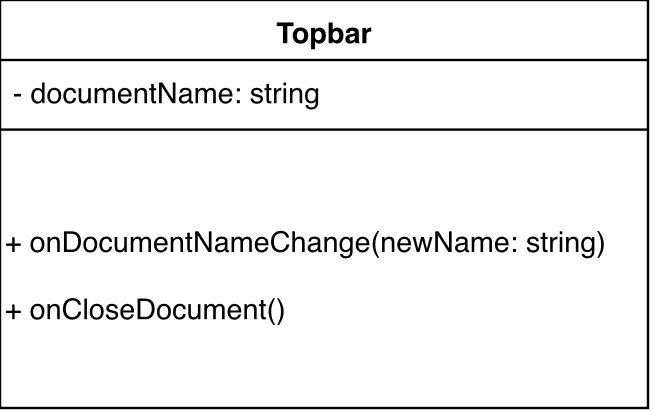
\includegraphics[width=0.8\textwidth]{../UMLimg/Topbar.jpg}
    \caption{UML TopBar}
    \label{fig:uml_topbar}
\end{figure}

% PROPS (invece di attributi e metodi i componenti hanno dati e funzioni di callback nella props)
\paragraph{Props (Dati)}
\begin{itemize}
    \item \texttt{documentName: string} - nome attuale del documento in fase di editing.
\end{itemize}

\paragraph{Props (Callback)}
\begin{itemize}
    \item \texttt{onDocumentNameChange: (newName: string) => void} - funzione invocata alla modifica del titolo.
    \item \texttt{onCloseDocument: () => void} - funzione invocata per chiudere il documento corrente.
\end{itemize}


\subsubsection{Sidebar}
Barra laterale contenente i pulsanti di navigazione (switch tra editor e storico) e per le funzionalità operative (salvataggio, upload, stampa e azioni AI). Delega l'orchestrazione delle disabilitazioni (es. bloccare i bottoni AI quando si visualizza lo storico) tramite la logica della pagina padre.

\begin{figure}[H]
    \centering
    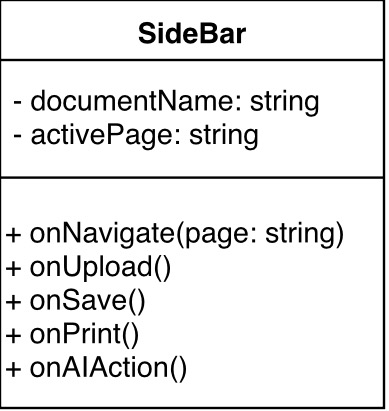
\includegraphics[width=0.8\textwidth]{../UMLimg/Sidebar.jpg}
    \caption{UML SideBar}
    \label{fig:uml_sidebar}
\end{figure}

\paragraph{Props (Dati)}
\begin{itemize}
    \item \texttt{activePage: 'editor' | 'history'} - determina la tipologia di view attualmente attiva per evidenziare il menu corretto (EditorPage o HistoryPage).
\end{itemize}

\paragraph{Props (Callback)}
\begin{itemize}
    \item \texttt{onNavigate: (page: 'editor' | 'history') => void} - aggiorna la view visualizzata.
    \item \texttt{onUpload: () => void} - innesca il caricamento di un file locale.
    \item \texttt{onSave: () => void} - innesca il flusso di salvataggio/esportazione.
    \item \texttt{onPrint: () => void} - invoca la stampa del documento.
    \item \texttt{onAiAction: () => void} - apre il pannello delle azioni di Intelligenza Artificiale.
\end{itemize}


\subsubsection{EditorButton}
Componente atomico e riutilizzabile che definisce l'interfaccia standard per tutti i bottoni della \texttt{Sidebar}. Gestisce i propri stati visivi (\texttt{isActive}, \texttt{disabled}) usando classi generate tramite \gls{CSS Modules}.

\begin{figure}[H]
    \centering
    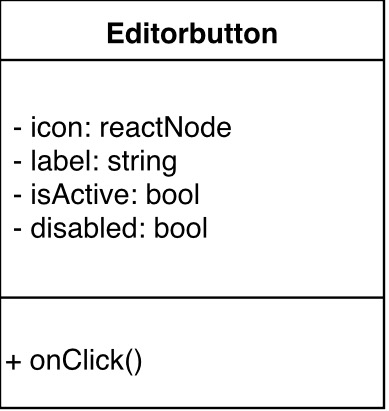
\includegraphics[width=0.8\textwidth]{../UMLimg/EditorButton.jpg}
    \caption{UML EditorButton}
    \label{fig:uml_editorButton}
\end{figure}

\paragraph{Props (Dati)}
\begin{itemize}
    \item \texttt{icon: ReactNode} - asset vettoriale/icona del bottone.
    \item \texttt{label: string} - etichetta testuale descrittiva.
    \item \texttt{isActive?: boolean} - determina lo stile di selezione.
    \item \texttt{disabled?: boolean} - inibisce l'interazione e applica lo stile di blocco.
\end{itemize}

\paragraph{Props (Callback)}
\begin{itemize}
    \item \texttt{onClick: () => void} - gestisce l'evento di pressione sul bottone.
\end{itemize}


\subsubsection{MarkdownEditor}
Componente delegato al rendering del corpo principale dell'area di scrittura. Consiste in un wrapper reattivo attorno a una \texttt{textarea} nativa su cui l'istanza di \gls{EasyMDE} viene "agganciata" dal ViewModel. Gestisce autonomamente gli eventi di trascinamento (\textit{drag-and-drop}) dei file esterni.

\begin{figure}[H]
    \centering
    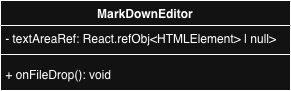
\includegraphics[width=0.8\textwidth]{../UMLimg/MarkDownEditor.jpg}
    \caption{UML MarkDownEditor}
    \label{fig:uml_markdownEditor}
\end{figure}

\paragraph{Props (Dati)}
\begin{itemize}
    \item \texttt{textAreaRef: \gls{React}.RefObject<HTMLTextAreaElement | null>} - puntatore fisico al nodo DOM su cui istanziare la libreria esterna.
\end{itemize}

\paragraph{Props (Callback)}
\begin{itemize}
    \item \texttt{onFileDrop?: (file: File) => void} - intercetta il rilascio di un file sull'area di testo.
\end{itemize}


\subsubsection{SaveDocumentModal}
Modale interattiva per la configurazione dell'esportazione del documento. Mantiene traccia dello stato locale (formato selezionato, modifiche al nome) e applica tecniche di \textit{sanitizzazione} sul testo immesso prima di confermare.

\begin{figure}[H]
    \centering
    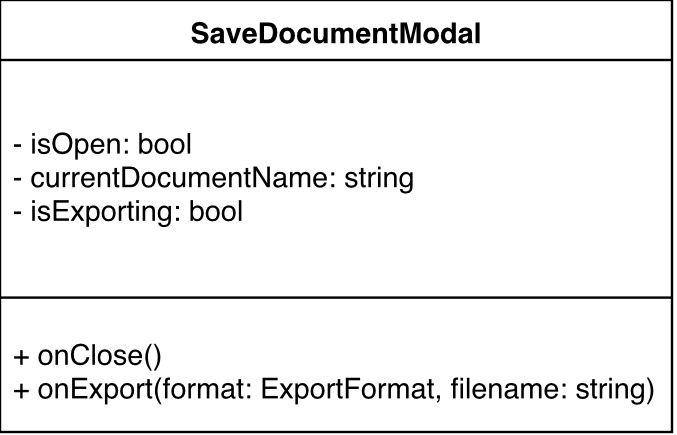
\includegraphics[width=0.8\textwidth]{../UMLimg/SaveDocumentModal.jpg}
    \caption{UML SaveDocumentModal}
    \label{fig:uml_saveDocumentModal}
\end{figure}

\paragraph{Props (Dati)}
\begin{itemize}
    \item \texttt{isOpen: boolean} - controlla la visibilità a schermo.
    \item \texttt{currentDocumentName: string} - funge da valore predefinito e \textit{placeholder} nell'input text.
    \item \texttt{isExporting?: boolean} - stato transitorio che disabilita i controlli durante l'elaborazione del download.
\end{itemize}

\paragraph{Props (Callback)}
\begin{itemize}
    \item \texttt{onClose: () => void} - innesca la chiusura senza salvataggio.
    \item \texttt{onExport: (format: ExportFormat, filename: string) => void} - passa i parametri sanitizzati al ViewModel per l'esecuzione del salvataggio.
\end{itemize}


\subsubsection{AiPanel}
% descrizione
% grafico
\paragraph{Props (Dati)}
\paragraph{Props (Callback)}


\subsubsection{AiWidget}
% descrizione
% grafico
\paragraph{Props (Dati)}
\paragraph{Props (Callback)}


\subsubsection{HistoryList}
Componente per il rendering aggregato dello storico delle generazioni degli LLM. Gestisce internamente l'alternanza visiva tra stati di transizione (caricamento, errore) e lo stato di successo, delegando la visualizzazione del singolo nodo a \texttt{HistoryCard}.

\subsection{HistoryList}
\begin{figure}[H]
    \centering
    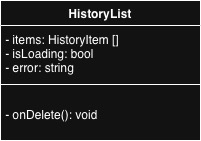
\includegraphics[width=0.8\textwidth]{../UMLimg/HistoryList.jpg}
    \caption{UML HistoryList}
    \label{fig:uml_historyList}
\end{figure}

\paragraph{Props (Dati)}
\begin{itemize}
    \item \texttt{items: HistoryItem[]} - array di oggetti rappresentanti le generazioni AI.
    \item \texttt{isLoading: boolean} - abilita il rendering dell'indicatore di caricamento.
    \item \texttt{error: string | null} - stringa che riporta un messaggio d'errore nel caricamento della cronologia (se presente).
\end{itemize}

\paragraph{Props (Callback)}
\begin{itemize}
    \item \texttt{onDelete: (id: string) => void} - propaga verso l'alto la richiesta di rimozione di uno specifico elemento.
\end{itemize}


\subsection{HistoryCard}
Componente granulare che rappresenta la singola scheda di interazione AI. Incapsula logiche puramente visive tramite \texttt{useState}, quali l'espansione/compressione di testi lunghi e il feedback del pulsante di copia negli appunti (\textit"Copiato!").

\begin{figure}[H]
    \centering
    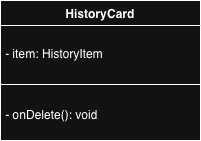
\includegraphics[width=0.8\textwidth]{../UMLimg/HistoryCard.jpg}
    \caption{UML HistoryCard}
    \label{fig:uml_historyCard}
\end{figure}

\paragraph{Props (Dati)}
\begin{itemize}
    \item \texttt{item: HistoryItem} - struttura dati completa dell'interazione (\gls{prompt}, output, modello usato, data).
\end{itemize}

\paragraph{Props (Callback)}
\begin{itemize}
    \item \texttt{onDelete: (id: string) => void} - gestisce l'eliminazione di una card specifica.
\end{itemize}


\newpage
% ============
% VIEW-MODEL
% ============
\subsection{ViewModel: custom hooks e logica di business}
Il ViewModel funge da intermediario tra il Model e la View ed è implementato tramite \textbf{Custom Hooks} specializzati. Ogni hook rispetta il \textit{Single Responsibility Principle} (SRP).
Il ViewModel ha la responsabilità di:
\begin{itemize}
    \item Esporre i dati e lo stato degli store alle View in un formato pronto per la visualizzazione.
    \item Gestire la logica di interazione complessa (ad esempio, l'orchestrazione delle \gls{API} AI tramite la Facade \texttt{aiCall}).
    \item Manipolare direttamente le istanze di librerie esterne, come \textbf{\gls{EasyMDE}} per l'editor \gls{Markdown}, isolandone la complessità tecnica all'interno di hook dedicati.
\end{itemize}

% descrizione degli hooks singoli
\subsubsection{useEditor}
Hook centrale dell'applicazione. Gestisce il ciclo di vita dell'istanza \gls{EasyMDE} (creazione al mount, distruzione al cleanup). Implementa l'auto-save con tecnica di \textit{debounce} (500 ms) per evitare scritture eccessive su disco. Fornisce all'esterno un'interfaccia solida per interagire con il testo.

% GRAFICO
\begin{figure}[H]
    \centering
    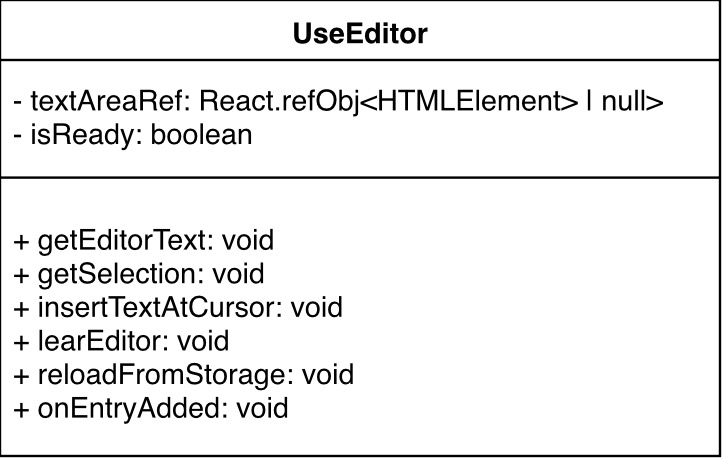
\includegraphics[width=0.8\textwidth]{../UMLimg/UseEditor.jpg}
    \caption{UML UseEditor}
    \label{fig:uml_useEditor}
\end{figure}

\paragraph{Stato/Valori di ritorno}
\begin{itemize}
    \item \texttt{textAreaRef: \gls{React}.RefObject<HTMLTextAreaElement | null>} - riferimento iniettato nella view.
    \item \texttt{isReady: boolean} - \textit{flag} che indica la completa inizializzazione del motore di rendering \gls{Markdown}.
\end{itemize}

\paragraph{Funzioni esposte}
\begin{itemize}
    \item \texttt{getEditorText: () => string} - restituisce l'intero contenuto testuale corrente.
    \item \texttt{getSelection: () => string} - estrae la porzione di testo evidenziata dall'utente.
    \item \texttt{insertTextAtCursor: (text: string) => void} - inietta testo elaborato (es. output AI) nella posizione attuale del cursore.
    \item \texttt{clearEditor: () => void} - resetta l'area di lavoro.
    \item \texttt{reloadFromStorage: () => void} - forza la sincronizzazione con il LocalStorage.
\end{itemize}


\subsubsection{useSaveDocument}
Coordina il flusso di esportazione asincrono. Orchestra in sequenza la composizione sicura del filename, il download fisico (mediato dal file \texttt{fileHandler.ts}) e il dispatch verso lo store per aggiornare il timestamp di salvataggio. In caso di errore fallisce silenziosamente mantenendo la modale aperta per un nuovo tentativo.

% grafico

\paragraph{Stato/Valori di ritorno}
\begin{itemize}
    \item \texttt{isOpen: boolean} - stato di visibilità della modale di salvataggio.
    \item \texttt{isExporting: boolean} - stato transitorio che indica se il processo di download è in corso.
\end{itemize}

\paragraph{Funzioni esposte}
\begin{itemize}
    \item \texttt{openModal: () => void} - innesca l'apertura della modale.
    \item \texttt{closeModal: () => void} - innesca la chiusura della modale.
    \item \texttt{handleExport: (rawFilename: string, format: ExportFormat, content: string) => Promise<void>} - processa la richiesta di esportazione, applica la mappa dei MIME type ed esegue il download.
\end{itemize}


\subsubsection{useFileUpload}
Gestisce il caricamento asincrono tramite \texttt{FileReader}. Esegue controlli preventivi (\gls{validazione} del formato supportato \texttt{.md} o \texttt{.txt}, dimensione massima 5 MB) e previene la perdita accidentale di dati non salvati bloccando l'utente e chiedendogli conferma tramite \texttt{window.confirm}.

% grafico

\paragraph{Stato/Valori di ritorno}
\begin{itemize}
    \item \texttt{fileInputRef: \gls{React}.RefObject<HTMLInputElement>} - riferimento fisico all'input nascosto di tipo \texttt{file} nel DOM.
\end{itemize}

\paragraph{Funzioni esposte}
\begin{itemize}
    \item \texttt{triggerFileInput: () => void} - simula il click sull'input nascosto per aprire la finestra di dialogo di sistema.
    \item \texttt{handleFileUpload: (event: \gls{React}.ChangeEvent<HTMLInputElement>) => Promise<void>} - intercetta il file selezionato, lo valida e ne legge il contenuto testuale.
\end{itemize}


\subsubsection{usePrintDocument}
Isola e rende testabile la logica di invocazione della stampa di sistema (\texttt{window.print()}). Implementa \textit{guard clauses} per impedire l'avvio del processo se il documento risulta vuoto.
Questo hook opera esclusivamente in modo imperativo, non ha quindi nessuno stato locale esposto.

% grafico

\paragraph{Funzioni esposte}
\begin{itemize}
    \item \texttt{handlePrint: (content: string) => void} - \gls{verifica} la lunghezza del contenuto e innesca la stampa del browser o genera un errore visivo.
\end{itemize}


\subsubsection{useHistory}
Interfaccia la View con lo store dedicato (\texttt{useHistoryStore}), estraendo le interazioni passate. Per garantire alte prestazioni e fluidità UI, tramite \texttt{useMemo} applica dinamicamente i filtri di ricerca e l'ordinamento cronologico, assicurando che lo strato di presentazione riceva sempre informazioni formattate senza subire calcoli ridondanti.

% grafico

\paragraph{Stato/Valori di ritorno}
\begin{itemize}
    \item \texttt{entries: HistoryEntry[]} - array delle interazioni, eventualmente filtrato e ordinato in base ai criteri correnti.
    \item \texttt{isLoading: boolean} - indica se i dati sono ancora in fase di recupero dal LocalStorage o dallo store.
    \item \texttt{error: string | null} - eventuale stringa di errore occorso durante il fetching della history.
\end{itemize}

\paragraph{Funzioni esposte}
\begin{itemize}
    \item \texttt{deleteEntry: (id: string) => void} - innesca la cancellazione di una specifica riga dallo storico persistente.
\end{itemize}


\subsubsection{useAiOperations}
% descrizione
% grafico
\paragraph{Stato/Valori di ritorno}
\paragraph{Funzioni esposte}


\newpage
% DEPENDENCY INJECTION
\subsection{Dependency Injection}
A legare i tre strati architetturali intervengono le \textbf{Page} (\texttt{EditorPage} e \texttt{HistoryPage}). Questi componenti non appartengono né alla View pura né al ViewModel, ma fungono da \textbf{Orchestratori}.

L'\texttt{EditorPage}, ad esempio, istanzia tutti i ViewModel necessari (\texttt{useEditor}, \texttt{useSaveDocument}, ecc.), legge lo stato dal Model e lo inietta nelle View. 

Un principio trasversale adottato è la \textbf{Dependency Injection}: per evitare un forte accoppiamento, i ViewModel non si importano a vicenda. Ad esempio, \texttt{useEditor} non importa la logica dello storico, ma riceve una callback \texttt{onEntryAdded} passata dall'orchestratore. Questo approccio garantisce che ogni hook sia testabile in totale isolamento fornendo semplicemente dei \textit{mock} in fase di testing.


\newpage

\section{Design pattern}
La progettazione del sistema \textit{Second Brain} ha fatto largo uso di design pattern orientati agli oggetti e funzionali, al fine di garantire un basso accoppiamento e un'alta coesione del codice.

\subsubsection{Facade pattern}
Per la gestione delle comunicazioni HTTP con il backend, il sistema applica il \textbf{Pattern Facade} a due livelli sovrapposti, ciascuno con una responsabilità architetturale distinta. I ViewModel e i componenti della View non invocano mai direttamente la libreria esterna \texttt{Axios}; al contrario, si interfacciano con moduli dedicati che nascondono la complessità delle transazioni di rete dietro un'interfaccia unificata.

\paragraph{Livello 1: \texttt{apiClient.ts} (Configurazione e normalizzazione)}
Il primo livello costituisce la Facade sull'istanza di \texttt{Axios}. È responsabile di:
\begin{itemize}
    \item \textbf{Configurazione centralizzata}: Risolve dinamicamente la \texttt{baseURL} dalle variabili d'ambiente (\texttt{\gls{VITE}\_API\_BASE\_URL}), con \textit{fallback} a \texttt{/\gls{api}}, e imposta il timeout (\texttt{\gls{VITE}\_API\_TIMEOUT}, default 30.000 ms). Garantisce che un unico punto del codice controlli i parametri di connessione.
    \item \textbf{Normalizzazione degli errori}: Tramite un \textit{response interceptor}, tutte le eccezioni di rete (timeout, errori HTTP 4xx/5xx, richieste annullate tramite \texttt{AbortSignal}) vengono intercettate e trasformate in oggetti \texttt{Error} standard. La logica di normalizzazione è incapsulata nella funzione pura \texttt{transformApiError}, testabile in totale isolamento.
    \item \textbf{Gestione della cancellazione}: Il supporto nativo all'\texttt{AbortSignal} permette ai ViewModel di annullare richieste in corso (es. operazione AI interrotta dall'utente) passando il segnale nella configurazione della chiamata.
\end{itemize}
L'interfaccia \texttt{ApiError} esportata definisce il contratto atteso per le risposte di errore del backend \gls{Flask}, garantendo una tipizzazione statica sicura su tutta la catena di chiamate.

\paragraph{Livello 2: \texttt{aiCall.ts} (Astrazione dell'\gls{endpoint} AI)}
Il secondo livello rappresenta una Facade sull'\textit{\gls{endpoint} specifico} del backend. Nasconde l'URL esatto (\texttt{/ai/generate}) e la struttura del payload JSON, esponendo una singola funzione asincrona:

\begin{verbatim}
executeOperation(payload: AiRequestPayload, signal?: AbortSignal)
    : Promise<string>
\end{verbatim}

Il tipo \texttt{AiOperationId} enumerato in questo modulo costituisce il contratto tipizzato tra frontend e backend: ogni identificatore (es. \texttt{"summary"}, \texttt{"white\_hat"}) corrisponde a una chiave dell'\texttt{OPERATION\_REGISTRY} lato server, garantendo che il frontend non possa inviare comandi non riconosciuti.

\paragraph{Architettura a cascata e vantaggi}
I due livelli formano una \textbf{Facade a cascata} con responsabilità rigorosamente separate:
\begin{itemize}
    \item \texttt{apiClient}: Sa \textit{come} parlare con il server (timeout, header, normalizzazione). Non conosce il dominio applicativo (Intelligenza Artificiale).
    \item \texttt{aiCall}: Sa \textit{dove} inviare la richiesta (\texttt{/ai/generate}) e \textit{cosa} spedire. Non conosce i dettagli implementativi di \texttt{Axios}.
    \item \textbf{ViewModel} (es. \texttt{useAiOperations}): Sanno \textit{quando} chiamare l'AI e come gestire il risultato nella UI. Non conoscono né \texttt{Axios} né l'URL dell'\gls{endpoint}.
\end{itemize}

Questa separazione porta due benefici misurabili in termini di qualità del software:
\begin{enumerate}
    \item \textbf{Disaccoppiamento tecnologico}: L'applicazione è agnostica rispetto al client HTTP. Una futura migrazione all'\gls{API} nativa \texttt{fetch} richiederebbe modifiche unicamente al file \texttt{apiClient.ts}, lasciando intatti tutti gli hook e i componenti.
    \item \textbf{Testabilità tramite mocking}: Nei test di unità eseguiti con \gls{Vitest}, isolare la logica di rete è immediato: è sufficiente fornire un \textit{mock} di \texttt{executeOperation} senza dover intercettare richieste HTTP reali, rendendo i test deterministici e veloci.
\end{enumerate}

% grafico

\newpage

% STRATEGY
\subsection{Pattern comportamentali: Strategy pattern}
Il design pattern comportamentale Strategy definisce una famiglia di algoritmi, li incapsula in classi separate e li rende intercambiabili in modo dinamico.

\subsubsection{Problema}
L’architettura iniziale del backend presentava un'eccessiva complessità logica dovuta alla gestione di molteplici modelli LLM e diverse logiche di prompting. La presenza di numerosi blocchi condizionali (if/else o switch) all'interno dell'entry point (\texttt{app.py}) rendeva il codice rigido, difficile da scalare e violava il principio di singola responsabilità (Single Responsibility Principle).

\subsubsection{Applicazione: \gls{prompt} strategies (ai\_strategies.py)}
Questa prima applicazione del pattern gestisce la trasformazione del testo grezzo fornito dall'utente in un input strutturato e ottimizzato per l'IA.

\paragraph{BaseAIStrategy}
Definisce il contratto comune per tutte le strategie di generazione dei \gls{prompt}.
\textbf{Proprietà e metodi:}
\begin{itemize}
    \item \texttt{temperature}: Definisce il livello di creatività dell'output (es. valori più alti per operazioni creative, più bassi per task analitici).
    \item \texttt{build(text: str)}: Impone a ogni sottoclasse di restituire una tupla contenente due stringhe: il \gls{System prompt} (il ruolo dell'IA) e lo \gls{User prompt} (il task specifico).
\end{itemize}

\paragraph{SimplePromptStrategy}
Utilizzata per le operazioni editoriali standard (riassunto, correzione grammaticale, riscrittura, \gls{distant writing}). Costruisce \gls{prompt} diretti impostando un ruolo e istruzioni ferree per evitare preamboli discorsivi nella risposta dell'IA.
\\ \textbf{Attributi:}
\begin{itemize}
    \item \texttt{role} (str): Definisce l'identità dell'assistente (es. "Sei un correttore di bozze").
    \item \texttt{task} (str): Definisce l'istruzione specifica da eseguire.
\end{itemize}

\paragraph{TranslationStrategy} 
Sottoclasse concreta specializzata nella gestione delle attività di traduzione multilingua. Questa classe ottimizza il \gls{prompt} per garantire che l'LLM operi esclusivamente come traduttore professionale, mantenendo la fedeltà linguistica.\\
\textbf{Attributi:}
\begin{itemize}
    \item language(str): Stringa che definisce la lingua di destinazione (es. "inglese", "cinese mandarino"). Questo attributo viene utilizzato per parametrizzare dinamicamente la richiesta al modello.
\end{itemize}
\textbf{Metodi:}
\begin{itemize}
    \item build(text): Implementa la logica di costruzione del \gls{prompt} impostando un \gls{System \gls{Prompt}} rigido che definisce il ruolo (traduttore professionista) e i vincoli di output (nessuna frase introduttiva). Lo \gls{User \gls{Prompt}} include l'istruzione di traduzione specifica verso la lingua memorizzata nell'attributo language.
\end{itemize}

\paragraph{DeBonoHatStrategy}
Sottoclasse concreta progettata per implementare il metodo dei "Sei Cappelli per Pensare" di Edward de Bono. Questa strategia guida l'LLM verso un'analisi laterale e strutturata, forzando il modello a osservare il testo da una singola prospettiva cognitiva alla volta (emotiva, logica, creativa, ecc.).\\
\textbf{Attributi:}
\begin{itemize}
    \item hat\_name(str): Memorizza il nome o il colore del cappello. Serve a definire l'identità dell'IA.
    \item focus(str): Memorizza l'area di analisi specifica. Serve a guidare il focus del modello durante la generazione.
\end{itemize}
\textbf{Metodi:}
\begin{itemize}
    \item build(self, text): Utilizza le f-string per iniettare i valori di hat\_name e focus all'interno dei \gls{prompt}.
\end{itemize}

\subsubsection{Applicazione: model strategies
(model\_strategies.py)}
Questa seconda applicazione del pattern isola completamente i dettagli tecnici (\gls{Endpoint}, \gls{API} Keys, payload JSON) necessari per comunicare con i diversi provider di Intelligenza Artificiale.

\paragraph{AIModelStrategy} interfaccia comune per tutti i modelli linguistici IA.
\\ \textbf{Metodi:}
\begin{itemize}
    \item generate(self, system\_prompt, user\_prompt): Definisce il contratto per l'invocazione del modello. Ogni classe concreta deve implementare la logica specifica per inviare i \gls{prompt} al fornitore e restituire la risposta come stringa pulita.
\end{itemize}

\paragraph{Implementazioni concrete (ZucchettiLlamaStrategy e Gemma3Strategy)}
Il sistema prevede due implementazioni concrete che espongono in modo polimorfico i modelli \gls{Llama 3.2} (per operazioni standard e traduzioni) e \gls{Gemma 3} (per il pensiero laterale dei Sei Cappelli).
Entrambe le classi implementano la logica di chiamata \gls{API} (tramite modulo OpenAI compatibile), formattano la richiesta ed estraggono esclusivamente il contenuto testuale della risposta, isolandolo dai metadati di rete.\\
\textbf{Metodi:}
\begin{itemize}
    \item generate(system\_prompt, user\_prompt): Implementa la logica di chiamata \gls{API} tramite il modulo OpenAI, gestisce la struttura della richiesta inviando i due messaggi (System e User) nel formato richiesto dal protocollo ChatCompletion ed estrae e restituisce esclusivamente il contenuto testuale della risposta, isolandolo dai metadati della chiamata (come i token consumati o gli ID di richiesta).
\end{itemize}

\subsubsection{Caching (get\_model)}
La funzione \texttt{get\_model(model\_class)} gestisce un dizionario globale privato (\texttt{\_model\_instances}) per la memorizzazione delle istanze, che funge quindi da cache.
Quando il controller richiede una strategia di modello, la funzione \gls{verifica} se ne esiste già un'istanza nel dizionario: se non esiste, la crea e la salva; alle chiamate successive per la stessa classe, restituisce il riferimento già memorizzato. 
Questa soluzione architetturale ottimizza l'uso delle risorse prevenendo l'apertura di connessioni multiple non necessarie ai client \gls{API}.


\newpage

\subsection{Pattern creazionali}
\subsection{Registry pattern}
% non è più un registry, ma un mappa - DA MODIFICARE
Il pattern Registry funge da catalogo centralizzato e configuratore delle operazioni disponibili, disaccoppiando totalmente il Controller (\texttt{app.py}) dalla logica di creazione delle dipendenze.

\subsubsection{Problema}
L’integrazione tra le diverse strategie di prompting e i diversi LLM poneva un problema di accoppiamento rigido e di complessità gestionale. Senza un punto di coordinamento centrale, il Controller avrebbe dovuto:
\begin{itemize}
    \item Conoscere l'esistenza di tutte le classi concrete e importarle direttamente.
    \item Gestire manualmente la logica di accoppiamento tra \gls{prompt} e modelli.
    \item Contenere lunghi blocchi condizionali per istanziare la strategia corretta in base alla stringa ricevuta dal frontend.
\end{itemize}
Questa struttura avrebbe violato il principio di Inversione delle Dipendenze, rendendo l'aggiunta di una nuova operazione un processo rischioso e richiedendo la modifica del codice di routing principale ogni volta che viene introdotta una nuova funzionalità.

\subsubsection{Applicazione: operation\_registry.py}
Il modulo funge da punto di giunzione dell'intera architettura, orchestrando il legame tra le strategie di contenuto (\gls{prompt}) e le strategie di esecuzione (modelli).

\paragraph{OperationConfig} 
La struttura \texttt{OperationConfig} è definita tramite il decoratore \texttt{@dataclass} ed è progettata per garantire un accoppiamento debole tra i componenti. Agisce come un contenitore che incapsula le dipendenze necessarie a ogni singola operazione.\\
\textbf{Attributi:}
\begin{itemize}
    \item \texttt{model\_class} (\texttt{Type[AIModelStrategy]}): è il riferimento al tipo della classe del modello da istanziare, la cui creazione effettiva è delegata al sistema di caching (\texttt{get\_model}) visto in precedenza.
    \item \texttt{\gls{prompt}\_strategy} (\texttt{BaseAIStrategy}): è un'istanza preconfigurata della strategia di \gls{prompt} specifica per quell'operazione.
\end{itemize}

\paragraph{OPERATION\_REGISTRY}
Il nucleo del pattern è implementato come un dizionario globale che associa identificatori testuali univoci (es. \texttt{"summary"}, \texttt{"green\_hat"}) a oggetti \texttt{OperationConfig}. Questa architettura garantisce tre proprietà fondamentali:
\begin{itemize}
    \item \textbf{Adesione al principio Open-Closed}: Per aggiungere una nuova funzionalità è sufficiente registrare una nuova riga nel dizionario di configurazione. Il codice del controller rimane del tutto inalterato, chiuso alle modifiche ma aperto alle estensioni.
    \item \textbf{Routing dinamico dei modelli}: Il registro permette di assegnare il modello LLM più adatto a una specifica operazione. Ad esempio, nel sistema le operazioni editoriali e di traduzione sono instradate nativamente su \gls{Llama 3.2}, mentre le logiche di pensiero laterale dei Sei Cappelli sono delegate a \gls{Gemma 3:4B}.
    \item \textbf{Robustezza e fallback}: In caso di operazione non riconosciuta o assente nel payload della richiesta, il sistema fornisce una configurazione di default in modo trasparente tramite la costante \texttt{DEFAULT\_OPERATION = "summary"}, sfruttando il metodo \texttt{.get()} del dizionario ed evitando crash dell'applicazione.
\end{itemize}


\newpage

\section{Tracciamento dei requisiti}
In questa sezione è stato riportato il tracciamento dei requisiti del progetto "Second Brain" con lo scopo di avere una panoramica completa sui requisiti stabiliti nel documento dell'\gls{Analisi dei Requisiti} v.2.0.0 e sul loro conseguimento.

\subsection{Notazione dei requisiti}
Il codice identificativo segue il formato:
\[
R[Importanza]-[Tipo]-[Numero]
\]
Dove le voci assumono i seguenti significati:

\begin{description}
    \item[Importanza] \hfill \\
    Indica il grado di priorità del requisito:
    \begin{itemize}
        \item \textbf{O (Obbligatorio):} Requisito esplicitamente richiesto dall'azienda Zucchetti. La sua mancata implementazione implica il fallimento degli obiettivi primari del progetto.
        \item \textbf{D (Desiderabile):} Requisito non strettamente vincolante ma che il gruppo si impegna ad implementare per migliorare il prodotto.
        \item \textbf{OP (Opzionale):} Requisito di priorità minore, la cui implementazione può essere rimandata.
    \end{itemize}
    
    \item[Tipo] \hfill \\
    Indica la natura del requisito:
    \begin{itemize}
        \item \textbf{F (Funzionale):} Descrive le funzionalità e i servizi che il sistema deve fornire.
        \item \textbf{V (Vincolo):} Descrive limitazioni tecnologiche, normative o implementative imposte esternamente.
        \item \textbf{Q (Qualità):} Descrive le caratteristiche qualitative del sistema (es. performance, sicurezza, manutenibilità).
    \end{itemize}
    
    \item[Numero] \hfill \\
    Un numero intero progressivo univoco per tipologia di requisito.
\end{description}

\subsection{Tracciamento dei requisti funzionali}
\begin{longtable}{|c|p{11cm}|c|}
\hline
\textbf{Codice} & \textbf{Descrizione} & \textbf{Stato}\\
\hline
\endhead
RO-F-1 & Il sistema deve fornire un’area di testo per l’inserimento e la modifica del testo con supporto alla sintassi \gls{Markdown} standard (CommonMark).& Soddisfatto\\
\hline
RO-F-2 & Il sistema deve informare l’utente con un messaggio in caso di perdita della connessione Internet durante l’utilizzo dell’editor. & ...\\
\hline
RO-F-3 & Il sistema deve informare l’utente con un messaggio se l’editor non risponde ai comandi.& ...\\
\hline
RO-F-4 & L'editor deve compilare la sintassi \gls{Markdown} in tempo reale. & Soddisfatto\\
\hline
RO-F-5 & Deve essere presente un'area di visualizzazione del documento formattato rispetto alla sintassi \gls{Markdown}. & Soddisfatto \\
\hline
RO-F-6 & Il sistema deve informare l'utente con un messaggio se il pannello di anteprima non si aggiorna correttamente. & ... \\
\hline
RO-F-7 & Il sistema deve permettere all'utente di selezionare porzioni di testo tramite mouse o tastiera. & Soddisfatto \\
\hline
RO-F-8 & Il sistema deve permettere all'utente di modificare porzioni di testo selezionate. & Soddisfatto \\
\hline
RO-F-9 & Il sistema deve permettere all'utente di copiare una parte di testo selezionato. & Soddisfatto \\
\hline
RO-F-10 & Il sistema deve permettere all'utente di incollare un testo nell'area di testo. & Soddisfatto \\
\hline
RO-F-11 & Il sistema deve permettere all'utente di tagliare il testo selezionato. & Soddisfatto \\
\hline
RO-F-12 & Il sistema deve permettere all'utente di annullare l'ultima modifica effettuata. & Soddisfatto \\
\hline
RO-F-13 & Se non sono presenti operazioni annullabili, il sistema non esegue alcuna azione al comando Undo. & Soddisfatto \\
\hline
RO-F-14 & Il sistema deve permettere all'utente di ripristinare le modifiche precedentemente annullate. & Soddisfatto \\
\hline
RO-F-15 & Se non sono presenti operazioni ripristinabili, il sistema non esegue alcuna azione al comando Redo. & Soddisfatto \\
\hline
RO-F-16 & Nell'editor deve essere presente una barra degli strumenti (\gls{toolbar}) per applicare formattazioni \gls{Markdown} senza scrivere manualmente la sintassi. & Soddisfatto \\
\hline
RO-F-17 & Il sistema deve permettere l'applicazione del grassetto al testo tramite \gls{toolbar}. & Soddisfatto \\
\hline
RO-F-18 & Il sistema deve permettere l'applicazione del corsivo al testo tramite \gls{toolbar}. & Soddisfatto \\
\hline
RO-F-19 & Il sistema deve permettere l'applicazione della sottolineatura al testo tramite \gls{toolbar}. & Soddisfatto\\
\hline
RO-F-20 & Il sistema deve permettere di creare intestazioni tramite \gls{toolbar}. & Soddisfatto\\
\hline
RO-F-21 & Il sistema deve permettere l'inserimento di elementi di struttura (tabelle, separatori orizzontali) tramite \gls{toolbar}. & Soddisfatto\\
\hline
RO-F-22 & Il sistema deve permettere l'inserimento di liste numerate tramite \gls{toolbar}. & Soddisfatto\\
\hline
RO-F-23 & Il sistema deve permettere l'inserimento di elenchi puntati tramite \gls{toolbar}. & Soddisfatto\\
\hline
RO-F-24 & Il sistema deve permettere l'inserimento di link e riferimenti tramite \gls{toolbar}. & Soddisfatto \\
\hline
RO-F-25 & L'utente può applicare più stili contemporaneamente (es. grassetto, corsivo, sottolineatura) alla stessa sezione di testo. & Soddisfatto \\
\hline
RO-F-26 & L'utente può annullare una formattazione di una porzione di testo selezionato riapplicandola dalla \gls{toolbar}. & Soddisfatto \\
\hline
RO-F-27 & L'utente può estendere la formattazione a una porzione di testo parzialmente formattato riapplicandola dalla \gls{toolbar}. & Soddisfatto \\
\hline
RO-F-28 & L'utente può creare sottoliste attivando la creazione di una lista dalla \gls{toolbar} quando il cursore è già all'interno di una lista. & Soddisfatto \\
\hline
RO-F-29 & L'utente può scegliere una combinazione di formattazioni dalla \gls{toolbar} quando non è presente testo selezionato, per applicarle al testo che scriverà successivamente. & Soddisfatto \\
\hline
RO-F-30 & Il sistema deve permettere all'utente di selezionare porzioni di testo da inviare all'agente esterno. & Soddisfatto \\
\hline
RO-F-31 & Il sistema permette di inviare del testo ad un agente esterno. & ... \\
\hline
RO-F-32 & L'utente deve poter accedere alle azioni sul testo tramite agente esterno in ogni momento. & ... \\
\hline
RO-F-33 & Il testo generato viene prima mostrato come proposta, separata visivamente dal testo dell'utente. & ... \\
\hline
RO-F-34 & Il testo in stato di proposta include le opzioni di conferma, annullamento e rigenerazione. & ... \\
\hline
RO-F-35 & Il sistema non permette la modifica del testo generato mentre è in stato di proposta. & ... \\
\hline
RO-F-36 & Il testo generato dall'agente esterno, una volta confermato, viene inserito nella posizione del cursore se presente, altrimenti in fondo al testo. & ... \\
\hline
RO-F-37 & Una proposta che viene confermata viene inserita nel documento nell'editor e la sezione di proposta viene rimossa. & ... \\
\hline
RO-F-38 & Una volta generato e confermato, il testo dell'agente esterno è modificabile tramite le stesse funzionalità dell'editor disponibili per il testo utente. & ... \\
\hline
RO-F-39 & Una proposta annullata comporta la rimozione del testo generato dalla sezione di proposta e la rimozione della sezione stessa. & ... \\
\hline
RO-F-40 & Una proposta che viene rigenerata viene rimandata all'agente esterno con gli stessi parametri e la nuova risposta sovrascrive la proposta corrente. & ... \\
\hline
RO-F-41 & Il sistema deve informare l'utente con un messaggio in caso di errore durante la comunicazione con il servizio LLM. & ... \\
\hline
RO-F-42 & L'utente può annullare un'operazione AI in corso prima del suo completamento. & ... \\
\hline
RO-F-43 & In seguito all'annullamento di un'operazione AI, il documento rimane nello stato precedente alla richiesta. & ... \\
\hline
RO-F-44 & Se la generazione di testo si blocca prematuramente, rimane ciò che è già stato generato, in attesa che l'utente confermi, rigeneri o elimini la proposta. & ... \\
\hline
RO-F-45 & L'agente esterno applica modifiche esclusivamente al testo selezionato dall'utente. Un contesto aggiuntivo può essere fornito solo a scopo interpretativo e non deve essere alterato. & ... \\
\hline
RO-F-46 & L'utente può consultare il registro delle generazioni AI effettuate. & Soddisfatto \\
\hline
RO-F-47 & Il sistema deve gestire il caso in cui lo storico delle generazioni AI sia vuoto, informando l'utente con un messaggio appropriato. & Soddisfatto \\
\hline
RO-F-48 & Ogni generazione di testo dell'agente esterno viene inclusa nel registro delle generazioni, incluse quelle annullate dall'utente. & ... \\
\hline
RO-F-49 & Il sistema deve permettere all'utente di visualizzare il testo completo di una generazione dallo storico AI. & Soddisfatto \\
\hline
RO-F-50 & L'utente deve poter riassumere tutto o una parte selezionata del testo usando un agente esterno. & ... \\
\hline
RO-F-51 & L'utente deve poter usare un agente esterno per riscrivere tutto o una parte selezionata del testo migliorandolo seguendo determinate specifiche come sintassi, stile e chiarezza. & ... \\
\hline
RO-F-52 & L'utente deve poter tradurre il testo usando un agente esterno in: inglese, italiano, tedesco, francese, spagnolo e cinese mandarino. & ... \\
\hline
RO-F-53 & Se l'utente avvia una traduzione senza selezionare la lingua di destinazione, il sistema lo notifica e blocca l'operazione. & ... \\
\hline
RO-F-54 & Il sistema permette di avviare la correzione grammaticale del testo tramite agente esterno. & ... \\
\hline
RO-F-55 & Se non vengono rilevati errori grammaticali, il sistema informa l'utente dell'esito positivo della correzione. & ... \\
\hline
RO-F-56 & Il sistema consente all'utente di avviare l'analisi critica del testo selezionato o dell'intero documento utilizzando il cappello di De Bono scelto. & ... \\
\hline
RO-F-57 & Se il testo è insufficiente per l'analisi critica, il sistema notifica l'utente e interrompe l'operazione. & ... \\
\hline
RO-F-58 & Se l'utente avvia l'analisi critica senza selezionare un cappello di De Bono, il sistema lo notifica e blocca l'operazione. & ... \\
\hline
RO-F-59 & Il sistema permette l'invio di un \gls{prompt} scritto dall'utente per la generazione di testo tramite agente esterno. & ... \\
\hline
RO-F-60 & Il sistema permette la modifica del \gls{prompt} da inviare all'agente esterno prima dell'invio. & ... \\
\hline
RO-F-61 & L'agente esterno può generare testo basandosi su un \gls{prompt} fornitogli dall'utente. & ... \\
\hline
RO-F-62 & Se il \gls{prompt} fornito dall'utente è vuoto o incompleto, il sistema notifica l'utente e impedisce l'invio. & ... \\
\hline
RO-F-63 & L'utente può caricare un file dal proprio dispositivo all'interno dell'editor. & Soddisfatto \\
\hline
RO-F-64 & Il sistema deve supportare il caricamento di file in formato \gls{Markdown} (\texttt{.md}, \texttt{.\gls{markdown}}) e testo semplice (\texttt{.txt}). & Soddisfatto \\
\hline
RO-F-65 & Il sistema deve supportare il caricamento tramite dialogo di esplorazione file (file picker). & Soddisfatto \\
\hline
RO-F-66 & Prima di procedere con il caricamento di un file, il sistema chiede conferma all'utente. & Soddisfatto \\
\hline
RO-F-67 & Il sistema deve informare l'utente con un messaggio di esito (successo o errore) al termine di ogni tentativo di caricamento file. & Soddisfatto \\
\hline
RO-F-68 & Il sistema deve validare il formato del file selezionato e impedire il caricamento di formati non supportati. & ... \\
\hline
RO-F-69 & Il sistema deve validare le dimensioni del file selezionato e impedire il caricamento di file che superano la dimensione massima consentita. & ... \\
\hline
RO-F-70 & Il sistema deve impedire il caricamento di file corrotti o illeggibili. & ... \\
\hline
RO-F-71 & Il sistema deve permettere all'utente di rimuovere il file che ha caricato. & Soddisfatto \\
\hline
RO-F-72 & L'utente può annullare l'operazione di rimozione del file caricato, lasciando l'editor nel suo stato precedente. & ... \\
\hline
RO-F-73 & Il sistema deve essere in grado di convertire il documento da \gls{Markdown} al formato selezionato dall'utente. & Soddisfatto \\
\hline
RO-F-74 & Il sistema deve permettere di scaricare il file nel dispositivo dell'utente. & Soddisfatto\\
\hline
RO-F-75 & L'operazione di esportazione o stampa non deve alterare né chiudere il documento originale nell'editor. & Soddisfatto\\
\hline
RO-F-76 & Il sistema deve informare l'utente con un messaggio di esito al termine di ogni operazione di esportazione. & Soddisfatto \\
\hline
RO-F-77 & Il sistema deve consentire l'esportazione del documento in formato \gls{Markdown} (\texttt{.md}). & Soddisfatto \\
\hline
RO-F-78 & Il sistema deve controllare che il range di pagine inserito dall'utente sia valido (non superiore al numero di pagine del documento e non negativo). & ... \\
\hline
RO-F-79 & Il sistema deve permettere di collegare e inviare il documento a un dispositivo di stampa. & Soddisfatto \\
\hline
RO-F-80 & Il sistema deve informare l'utente con un messaggio in caso di errore durante l'invio del documento alla stampante. & Soddisfatto\\
\hline
RO-F-81 & Il sistema deve garantire la persistenza locale del testo nell'editor tramite browser storage (LocalStorage). & Soddisfatto\\
\hline
RO-F-82 & Il sistema deve garantire la persistenza locale dello storico delle generazioni AI tramite browser storage (\gls{Zustand} persist). & Soddisfatto \\
\hline
RO-F-83 & Il sistema deve impedire il caricamento di file di dimensioni superiori a 5MB. & Soddisfatto \\
\hline

% DESIDERABILI
RD-F-1 & Il sistema deve supportare l'uso di scorciatoie da tastiera per le operazioni di formattazione. & Soddisfatto \\
\hline
RD-F-2 & Il sistema deve permettere di cambiare modalità di visualizzazione (Solo Editor, Solo Anteprima, Split View). & Soddisfatto \\
\hline
RD-F-3 & Il sistema deve supportare il caricamento tramite drag-and-drop (trascinamento file nell'area dell'editor). & ... \\
\hline
RD-F-4 & Se sono presenti modifiche non salvate, il sistema chiede conferma all'utente prima di caricare un nuovo file. & Soddisfatto\\
\hline
RD-F-5 & Il parsing del contenuto del file caricato deve gestire caratteri non validi senza causare il crash dell'applicazione. & ... \\
\hline
RD-F-6 & I messaggi di errore relativi al caricamento file devono essere esplicativi e suggerire come procedere. & ... \\
\hline
RD-F-7 & Il sistema deve offrire più opzioni per le operazioni comuni sui file come carica nuovo, stampa, chiudi. & Soddisfatto \\
\hline
RD-F-8 & Il sistema deve consentire l'esportazione del documento in formato PDF. & ... \\
\hline
RD-F-9 & Il sistema deve consentire l'esportazione del documento in formato HTML. & Soddisfatto \\
\hline
RD-F-10 & Il sistema deve consentire l'esportazione del documento in formato ODT. & ... \\
\hline
RD-F-11 & Il sistema deve consentire l'esportazione del documento in formato DOCX. & ... \\
\hline
RD-F-12 & L'utente deve poter scegliere se esportare l'intero documento o un range di pagine selezionate. & Non soddisfatto \\
\hline
RD-F-13 & Il sistema deve consentire all'utente di scegliere il nome del file prima di procedere al download/esportazione. & Soddisfatto \\
\hline
RD-F-14 & Il sistema deve fornire un'anteprima del documento nel formato selezionato prima di procedere al download. & Non soddisfatto \\
\hline
RD-F-15 & Il sistema deve aprire il dialogo di stampa nativo del browser per configurare le opzioni di stampa. & Soddisfatto \\
\hline

% OPZIONALI
ROP-F-1 & L'utente può ricercare parole nel testo attraverso l'editor & ... \\
\hline
ROP-F-2 & Il sistema deve informare l'utente se la ricerca non ha prodotto occorrenze nel testo. & ... \\
\hline
ROP-F-3 & La sezione di testo generata come proposta è visibilmente diversa dal testo utente & Soddisfatto \\
\hline
ROP-F-4 & Per ogni voce del registro delle generazioni AI il sistema deve indicare la data e l'ora della generazione. & Soddisfatto \\
\hline
ROP-F-5 & Per ogni voce del registro delle generazioni AI il sistema deve indicare il tipo di operazione che ha prodotto la generazione. & Soddisfatto \\
\hline
ROP-F-6 & L'utente può eliminare una voce dal registro delle generazioni AI. & Soddisfatto \\
\hline
ROP-F-7 & Per gli utenti autenticati, il registro delle generazioni AI è persistente ed è associato ai documenti salvati nel proprio account. & Non soddisfatto \\
\hline
ROP-F-8 & La sezione di testo in stato di proposta viene colorata in base al tipo di operazione che viene fatta & Soddisfatto \\
\hline
ROP-F-9 & Il sistema deve visualizzare sia il testo originale che la traduzione generata, permettendo all'utente di confrontarle. & Soddisfatto \\
\hline
ROP-F-10 & Se il testo selezionato è già nella lingua di destinazione della traduzione, il sistema avvisa l'utente e interrompe l'operazione. & ... \\
\hline
ROP-F-11 & Il sistema offre esempi per la richiesta di generazione di testo a partire da un estratto & ... \\
\hline
ROP-F-12 & Il sistema permette di inserire un grafico generato, con dati presenti nel testo, scelto tra diversi tipi disponibili all'utente & Non soddisfatto \\
\hline
ROP-F-13 & Il sistema permette di inserire una tabella generata con dati presenti nel testo & Non soddisfatto \\
\hline
ROP-F-14 & Se i dati nel testo sono insufficienti per generare grafici o tabelle, il sistema notifica l'utente. & Non soddisfatto \\
\hline
ROP-F-15 & Il sistema permette di inserire una mappa concettuale generata con dati presenti nel testo & Non soddisfatto \\
\hline
ROP-F-16 & Se si verificano errori nella visualizzazione della mappa concettuale generata, il sistema notifica l'utente. & Non soddisfatto \\
\hline
ROP-F-17 & Il sistema permette di inserire una formula matematica generata con dati presenti nel testo & Non soddisfatto \\
\hline
ROP-F-18 & Se la formula matematica contiene simboli non supportati, il sistema notifica l'utente. & Non soddisfatto \\
\hline
ROP-F-19 & Il sistema deve permettere all'utente di inserire le proprie credenziali (username e password) per il login & Non soddisfatto \\
\hline
ROP-F-20 & Se le credenziali sono errate il sistema non permette all'utente di autenticarsi & Non soddisfatto \\
\hline
ROP-F-21 & Il sistema deve mostrare un messaggio di errore generico in caso di fallimento del login, senza specificare se l'errore riguarda username o password. & Non soddisfatto \\
\hline
ROP-F-22 & In caso di username già esistente durante la registrazione, il sistema deve proporre all'utente di effettuare il login o scegliere un nuovo username. & Non soddisfatto\\
\hline
ROP-F-23 & Il sistema deve permettere all'utente di potersi registrare tramite uno username e una password & Non soddisfatto \\
\hline
ROP-F-24 & Il sistema deve impedire la registrazione in caso ci sia uno username uguale nel \gls{database} & Non soddisfatto\\
\hline
ROP-F-25 & Il sistema deve salvare nel \gls{database} le password criptate in fase di registrazione & Non soddisfatto \\
\hline
ROP-F-26 & Il sistema deve permettere ad un \gls{utente autenticato} di poter eliminare il proprio account & Non soddisfatto \\
\hline
ROP-F-27 & Il sistema in caso di eliminazione account deve eliminare i dati dal \gls{database} & Non soddisfatto \\
\hline
ROP-F-28 & Le operazioni di eliminazione dell'account devono richiedere una conferma esplicita da parte dell'utente & Non soddisfatto \\
\hline
ROP-F-29 & Il sistema deve terminare la sessione se un account viene eliminato & Non soddisfatto \\
\hline
ROP-F-30 & L'utente può annullare la procedura di eliminazione del proprio account. & Non soddisfatto \\
\hline
ROP-F-31 & Il sistema deve permettere ad un utente di vedere i file che ha salvato & Non soddisfatto \\
\hline
ROP-F-32 & Il sistema deve permettere ad un \gls{utente autenticato} di selezionare un file dall'elenco di quelli salvati e aprirlo & Non soddisfatto \\
\hline
ROP-F-33 & Il sistema deve permettere all'utente di annullare l'operazione di apertura file, lasciando l'editor nel suo stato precedente. & Soddisfatto \\
\hline
ROP-F-34 & Il sistema deve mostrare i file salvati in ordine cronologico per data di ultima modifica. & Non soddisfatto \\
\hline
ROP-F-35 & L'accesso ai file salvati nel \gls{database} è consentito solo ad utenti autenticati. & Non soddisfatto \\
\hline
ROP-F-36 & Il sistema deve permettere il salvataggio di un file in un \gls{sistema di persistenza} non locale & Non soddisfatto \\
\hline
ROP-F-37 & Il sistema deve notificare l'utente in caso di fallimento del salvataggio nel \gls{database}. & Non soddisfatto \\
\hline
ROP-F-38 & Il sistema deve associare ogni file al suo creatore & Non soddisfatto \\
\hline
ROP-F-39 & Il sistema deve impedire il salvataggio di file nel \gls{database} da parte di utenti non autenticati. & Non soddisfatto \\
\hline
ROP-F-40 & Il sistema deve impedire il salvataggio di un documento vuoto nel \gls{database}. & Non soddisfatto \\
\hline
ROP-F-41 & Un \gls{utente non autenticato} che prova a salvare un file viene riportato alla pagina di login & Non soddisfatto \\
\hline
ROP-F-42 & L'utente può effettuare il logout in ogni momento e terminare la propria sessione & Non soddisfatto \\
\hline
ROP-F-43 & Il sistema deve permettere all'utente di modificare il nome del documento corrente direttamente dall'interfaccia di lavoro. & Soddisfatto \\
\hline
ROP-F-44 & Il sistema deve permettere all'utente di cercare testo all'interno del registro delle generazioni AI tramite una barra di ricerca. & Soddisfatto\\
\hline
ROP-F-45 & Il sistema deve permettere all'utente di filtrare le voci del registro delle generazioni AI in base al tipo di operazione effettuata. & Soddisfatto\\
\hline
\addlinespace[1em]
\caption{Tracciamento dei \gls{requisiti funzionali}}
\label{tab:tracciamento_requisiti_funzionali}
\end{longtable}

\subsection{Tracciamento dei requisti di qualità}
\begin{longtable}{|c|p{11cm}|c|}
\hline
\textbf{Codice} & \textbf{Descrizione} & \textbf{Stato}\\
\hline
\endhead
RO-Q-1 & Il tempo di risposta dell'interfaccia utente (aggiornamento anteprima, applicazione formattazioni) deve essere inferiore a 500 ms nel 95\% dei casi, misurato su una sessione utente attiva di almeno 30 minuti. & ... \\
\hline
RO-Q-2 & Il tempo medio di generazione di una risposta da parte del servizio LLM non deve superare i 10 secondi, misurato su un campione di almeno 20 richieste consecutive in condizioni di utilizzo normale.  & ... \\
\hline
RO-Q-3 & Il tasso di errori nelle operazioni principali (salvataggio, apertura file, chiamate AI) non deve superare l'1\%, misurato sul totale delle operazioni eseguite in una sessione utente attiva di almeno 30 minuti. & ... \\
\hline
RO-Q-4 & La percentuale di codice coperta dai test automatici (test coverage) deve essere almeno il 70\%, misurata sull'insieme completo dei moduli rilasciati ad ogni versione. & Soddisfatto \\
\hline
RO-Q-5 & La complessità ciclomatica (McCabe) di ogni funzione/metodo del codice prodotto non deve superare il valore 8. & ... \\
\hline
RO-Q-6 & La documentazione prodotta deve ottenere un Indice di Gulpease (IG) maggiore o uguale a 40. & Soddisfatto \\
\hline
RO-Q-7 & Il sistema deve essere sviluppato rispettando le Norme 
di Progetto del gruppo ByteMe. & Soddisfatto \\
\hline
RO-Q-8 & Il sistema deve essere verificato secondo il Piano di Qualifica prima di ogni rilascio. & Soddisfatto\\
\hline
RO-Q-9 & Il \gls{manuale utente} deve documentare tutte le funzionalità obbligatorie del sistema e deve ottenere un Indice di Gulpease (IG) maggiore o uguale a 40. & ... \\
\hline
RO-Q-10 & Il manuale di installazione e deployment del sistema deve ottenere un Indice di Gulpease (IG) maggiore o uguale a 40. & Soddisfatto \\
\hline
\addlinespace[1em]
\caption{Tracciamento dei \gls{requisiti di qualità}}
\label{tab:tracciamento_requisiti_qualità}
\end{longtable}

\subsection{Tracciamento dei requisti di vincolo}
\begin{longtable}{|c|p{11cm}|c|}
\hline
\textbf{Codice} & \textbf{Descrizione} & \textbf{Stato}\\
\hline
\endhead
RO-V-1 & L'applicazione deve essere accessibile tramite browser web. 
I browser supportati sono: Google Chrome ($\geq$ v110), Mozilla Firefox 
($\geq$ v110), Microsoft Edge ($\geq$ v110), Safari ($\geq$ v16). & ... \\
\hline
RO-V-2 & Il sistema deve utilizzare la codifica Unicode (UTF-8) per la rappresentazione interna e lo storage del testo. & Soddisfatto \\
\hline
RO-V-3 & Il formato di input e di storage del testo deve essere \gls{Markdown}, in conformità allo standard CommonMark. & Soddisfatto\\
\hline
RO-V-4 & Il sistema deve integrarsi con un servizio LLM tramite \gls{API} REST compatibili con lo standard OpenAI. & Soddisfatto \\
\hline
RO-V-5 & Il backend dell'applicazione deve essere progettato come un gateway \gls{stateless}; non deve mantenere sessioni o stati dei documenti sul server, delegando la gestione della persistenza interamente al client. & Soddisfatto \\
\hline
\addlinespace[1em]
\caption{Tracciamento dei \gls{requisiti di vincolo}}
\label{tab:tracciamento_requisiti_vincolo}
\end{longtable}

\end{document}
